\section{Introduction}
Nous avons présenté précédemment les concepts de base d'un système de reconnaissance de la parole, les travaux qui ont présenté les résultats les plus performants ainsi que la conception de \textit{ASeR-System}, notre système End-To-End de reconnaissance de la parole pour la langue arabe. En plus d'effectuer la tâche de reconnaissance, \textit{ASeR-System} est un environnement de développement permettant d'intégrer le système de reconnaissance, d'améliorer sa performance ou encore de développer un nouveau système, pour une autre langue par exemple.

Dans ce chapitre, nous commençons par présenter notre environnement de travail, les outils utilisés pour le développement et l'apprentissage, l'envoi des données, les résultats d'apprentissage ainsi que les performances des différents modèles, le teste de notre système de reconnaissance de la parole sur un système de questions-réponses et l'organisation de l'environnement de développement. 

\section{Environnement et outils de travail}
\subsection{Matériel}
La réalisation de ce projet s'est effectuée sur deux machines locales ainsi qu'un serveur cloud pour l'apprentissage des modèles. Nous avons opté pour un compte cloud Google Colaboratory \footnote{Google Colaboratory est un environnement de type "Jupyter Notebook" qui ne nécessite pas de configuration système et qui s'exécute entièrement sur le cloud \cite{colab}.}. Nous nous sommes tournés vers ce serveur cloud car il offre la puissance de calcul nécessaire en terme de GPU et plus particulièrement en terme de processeurs CUDA qui sont des unités de calcul massivement parallèles pour l'apprentissage profond. La configuration des deux machines locales ainsi que la machine virtuelle est présentée dans le tableau \ref{configMachines}.
\begin{center}
\begin{table}
    \centering
    \begin{tabular}{|c|c|c|c|}
        \hline 
        \rowcolor{lightgray}
        Paramétres & Machine 1 &  Machine 2 & Google Colaboratory  \\
        \hline
        \makecell{\textbf{Système}\\\textbf{d'exploitation}} & \makecell{GNU/Linux\\ Ubuntu}  & \makecell{macOS \\Mojave\\ 10.14.5}  & \makecell{Jupyter notebook-based system} \\
        \hline
        \makecell{\textbf{RAM}} & \makecell{8GO}  & \makecell{16GO}  & \makecell{13GO}\\
        \hline
        \makecell{\textbf{Processeur}} & \makecell{Intel Core\\ i7-8550 CPU \\}  & \makecell{2,9 GHz Intel\\Core i5}  & \makecell{2vCPU @ 2.2GHz}  \\
        \hline
        \makecell{\textbf{GPU}} & \makecell{-} & \makecell{-} & \makecell{1xTesla K80 @ 3.7 GHz \\ 2496 CUDA cores \\ 12GB GDDR5 VRAM}  \\
        \hline
    \end{tabular}
    \caption{Caractéristiques des machines utilisées}
    \label{configMachines}
\end{table}
\end{center}

\subsection{Langage de programmation et logiciels}
Afin d'implémenter notre système, il était nécessaire de choisir le langage de programmation ainsi que les différentes librairies que nous utilisons pour le développement et le test de notre système. Nous donnons dans cette section, une brève présentation de ces outils ainsi que leur utilité dans le cadre de ce projet. 

\subsubsection{Langage Python}
Python est un langage de programmation interprété, interactif et orienté objet. Il intègre des modules, des exceptions, du typage dynamique, des types de données dynamiques de très haut niveau et des classes. Python combine une puissance remarquable avec une syntaxe très claire \cite{python_lang}.

La syntaxe élégante et minimaliste, le grand nombre de bibliothèques scientifiques disponible en Open source ainsi que la grande communauté qui travaille dessus font de Python un langage idéal pour les scripts et le développement rapide d’applications dans de nombreux domaines et particulièrement le domaine de l'apprentissage automatique.

\subsubsection{Bibliothèques utilisées}

\begin{enumerate}
    \item \textbf{Pydub :} bibliothèque libre et Open source implémentée en python conçue pour manipuler un audio avec une interface simple et facile de haut niveau \cite{pydub}. Nous utilisons Pydub pour le découpage des enregistrements audio selon des temps de début et de fin de transcription. \\
    
    \item \textbf{Librosa :} disponible en libre accès pour l'analyse musicale ainsi que l'analyse audio. il fournit les éléments de base nécessaires à la création de systèmes de récupération d'informations audio \cite{librosa}. Nous utilisons librosa pour générer les spectoragmmes MFCC à partir des enregistrements audio.\\
    
    \item \textbf{NumPy (Numerical Python) :} est un package fondamental de calcul scientifique implémenté en Python et disponible en Open source. Ce package est essentiellement utilisé pour la manipulation des matrices ou tableaux multidimensionnels ainsi que des fonctions mathématiques opérant sur ces derniers. Au-delà de ses utilisations scientifiques évidentes, NumPy peut également être utilisé comme un conteneur multidimensionnel efficace de données génériques \cite{numpy}. Nous utilisons Numpy pour encapsuler les données pour qu'elles soient utilisées lors de l'apprentissage.\\
    
    \item \textbf{psutil (process and system utilities) :}  est une bibliothèque multiplate-forme permettant de récupérer des informations sur les processus en cours et l'utilisation du système en Python. Il est principalement utile pour la surveillance du système, l'établissement de profils et la limitation des ressources de processus et la gestion des processus en cours \cite{psutil}. Nous utilisons psutil pour lire la taille de la mémoire vive de l'utilisateur pour le partitionnement dynamique des datasets.\\
    
    \item \textbf{matplotlib :} bibliothèque de traçage Python 2D qui produit des images de qualité dans une variété de formats papier et d’environnements interactifs sur toutes les plateformes \cite{matplotlib}. Nous utilisons Matplotlib pour dresser les différentes courbes de performance lors des apprentissages. \\
    
    \item \textbf{TensorFlow :} plate-forme open source pour l'apprentissage automatique. Elle offre un écosystème complet et flexible d’outils, de bibliothèques et de ressources communautaires qui permet aux chercheurs de se familiariser avec les technologies de pointe et aux développeurs de créer et de déployer facilement des applications utilisant l'apprentissage automatique. \\
    
    \item \textbf{Keras :} API de réseaux de neurones de haut niveau écrite en Python et qui enveloppe les fonctionnalités de la bibliothèque Tensorflow. Keras permet d'avoir un prototypage simple et rapide (convivialité, modularité et extensibilité), il prend en charge les réseaux convolutionnels et les réseaux récurrents, ainsi que les combinaisons des deux \cite{keras}. \\
    
    \item \textbf{Lang-trans :} bibliothèque Python de translittération principalement à partir de scripts non latins tels que l'arabe, le japonais, etc. \cite{translang}. \\
    
    \item \textbf{PyAudio :} bibliothèque python permettant d'effectuer différentes manipulation sur l'audio \cite{PyAudio}. Nous utilisons PyAudio afin d'enregistrer un signal audio à partir du microphone de la machine. \\
    
    \item \textbf{PyQT :} bibliothèque python permettant de développer des interfaces graphiques \cite{pyqt}. Nous l'utilisons pour développer notre application de test.
\end{enumerate} 
\subsubsection{Formats de données}
\begin{enumerate}
    \item \textbf{Pickle :} module qui implémente des protocoles binaires pour sérialiser et dé-sérialiser une structure d'objet Python. «Pickling» est le processus par lequel une hiérarchie d'objets Python est convertie en un flux d'octets et «unpickling» est l'opération inverse, par laquelle un flux d'octets (à partir d'un fichier binaire ou d'un objet de type octet) est reconverti en une hiérarchie d'objets \cite{pickle} \label{pickle}. \\
    
    \item \textbf{XML (eXtensible Markup Language) : }  est une extension de format de fichier qui est similaire au HTML. Un fichier XML contient des symboles de balisage décrivant le contenu d'une page ou d'un fichier. XML est considéré comme extensible car les symboles de balisage sont illimités et se définissent d'eux-mêmes \cite{XML}. \\
    
    \item \textbf{wav :} Un fichier WAV est un fichier audio qui utilise un format audio numérique standard pour stocker des données. Il permet de sauvegarder les enregistrements audio avec différentes fréquences d’échantillonnage et différents débits binaires. Il est souvent sauvegardé dans un format stéréo à 44,1 KHz, 16 bits \cite{wav}.
\end{enumerate}

\subsubsection{Logiciels}
\begin{enumerate}
    \item \textbf{PyCharm :} environnement de développement intégré utilisé pour programmer en Python. Il fournit une assistance et analyse de codage, une navigation fluide dans le code, la prise en charge de framework web, etc. \cite{pycharm}. \\
    
    \item \textbf{Sublime Text :} est un éditeur de texte générique codé en C++ et Python. Il est disponible sur les trois systèmes d'exploitation à savoir Windows, Mac OS et Linux. L'éditeur prend en charge 44 langages de programmation majeurs \cite{sublime}. \\
    
    \item \textbf{Git :} est un système de contrôle de versions distribué gratuit et Open source, conçu pour gérer tout projet en équipe, du plus petit au plus grand, avec rapidité et efficacité \cite{git}.
\end{enumerate}


\section{Préparation des données pour l'apprentissage}
La préparation des données est une étape délicate qui affecte grandement les résultats de l'apprentissage selon la qualité du pré-traitement des données. Cela est d'autant plus vrai lorsque nous traitons des données de type séries temporelles et des corpus de très grande taille \cite{timeseriesdata} comme c'est le cas pour le développement d'un système de reconnaissance de la parole.

Nous présentons dans cette section comment nous avons effectué les tâches suivantes : 
\begin{itemize}
    \item extraction des transcriptions et partitionnement des longs enregistrements audio en enregistrements plus courts pour le corpus élargi,
    \item conversion des enregistrements audio et transcriptions en fichiers binaires de dix heures de dialogue chacun, et
    \item encodage basé caractères et basé mots des transcriptions.
\end{itemize}

\subsection{Traitement du corpus élargi}
Comme mentionné dans le chapitre de conception, le corpus élargi est un corpus proposé en libre accès par l'équipe QCRI \cite{mgb2corpus}. Ce corpus contient un total de 2214 enregistrements audio d'une durée qui varie entre 20 minutes et un peu plus d'une heure chacun. Ces derniers sont des enregistrements d'émissions télévisées de la chaîne Al Jazeera et contiennent plusieurs centaines de phrases et donc plusieurs centaines de transcriptions pour chaque fichier. Nous retrouvons, associé à ces fichiers audio, leurs transcriptions sous forme de fichiers XML contenant les temps de début et de fin de chaque transcription, l'identité de l'orateur et la liste de mots d'une transcription. La figure \ref{xml_exemple} est un exemple de transcription :

 \begin{figure}[H]
     \centering
     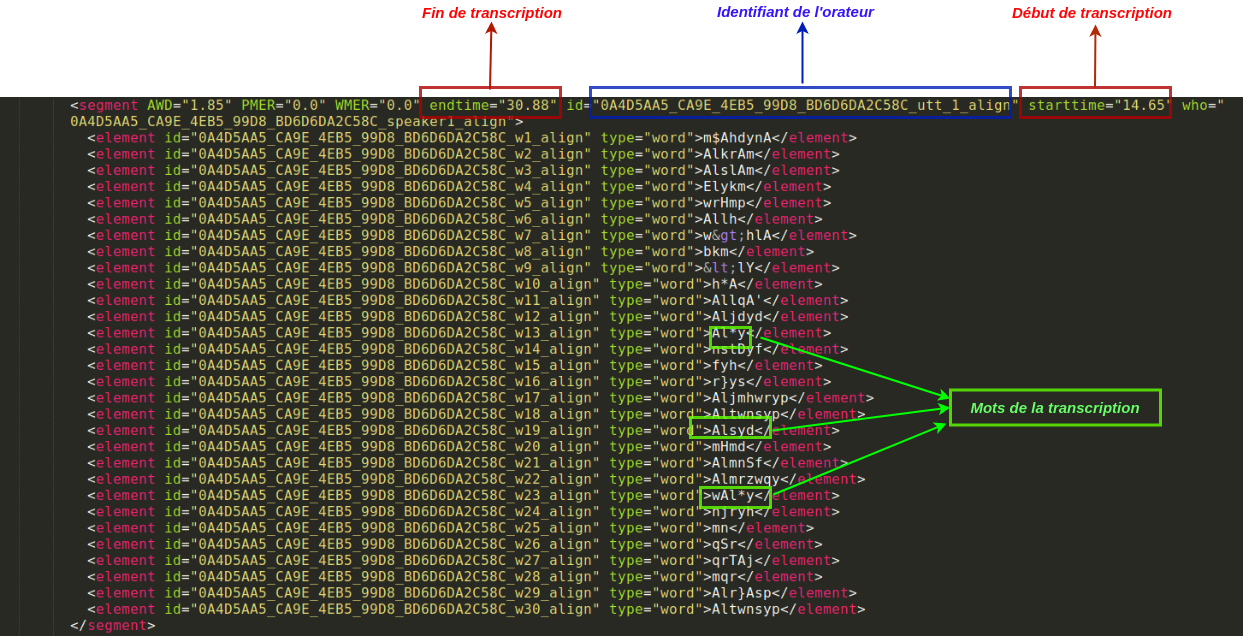
\includegraphics[width=400pt]{images/chap4/example_trans.png}
     \caption{Exemple de transcription dans un fichier XML du corpus élargi}
     \label{xml_exemple}
 \end{figure}
 
Nous implémentons donc l'algorithme que nous avons présenté dans la section \ref{collecte_donnees} en utilisant les méthodes de la bibliothèque Python "\textit{XML}" ainsi que les méthodes de la bibliothèque "\textit{Pydub}" pour effectuer le découpage des enregistrements audio selon les temps de début et fin d'enregistrement. 

 
\subsection{Conversion des fichiers audio et fichiers texte en dataset de dix heures}
Afin de rendre l'exploitation des données plus simple, mais surtout plus rapide, nous créons une classe que nous nommons \textit{"AudioInput"}. Cette classe aura pour but de contenir le spectrogramme de l'enregistrement, sa transcription, son chemin ainsi que sa durée. Ensuite, nous parcourons chaque couple de répertoires audio et fichier de transcriptions et appliquons les modifications liées aux caractères qui n'appartiennent pas à la table Buckwalter \cite{buckwalter} que nous avons citées dans la section \ref{trans_preprocessing}. Pour finir, nous définissons une limite de durée pour chaque dataset et générons des fichiers binaire de type \textit{Pickle} contenant une liste d'objets \textit{AudioInput} totalisant dix heures de dialogue.

Cette limite du nombre d'heures de dialogue pour chaque fichier Picke a pour but :
\begin{itemize}
    \item de simplifier l'upload des fichiers Pickle sur le cloud,
    \item d'éviter les dépassements de taille de mémoire vive lors de la génération de ces fichiers car nous libérons l'espace mémoire après avoir généré les dix heures,  
    \item de simplifier la séparation des datasets en données d'apprentissage et de test, et
    \item de faciliter la manipulation des datasets pour les 60 heures, 260 heures et 1200 heures d'apprentissage. \\
\end{itemize}

La génération de ce corpus est une opération qui a pris à la machine un total de quatre jours. Ce temps est due à la quantité de données à notre disposition, qui est de 118 GO, ainsi qu'à la durée de génération des spectrogrammes MFCC à l'aide de la bibliothèque \textit{Librosa}. Il est à noter que cette opération n'aurait pas pu se faire sans partitionnement des données à cause de la mémoire vive qui aurait été saturée. 

\subsection{Encodage des transcriptions}
Les réseaux de neurones ne traitent que les données numériques d'où la nécessité d'encoder les transcriptions sous forme de données numériques. Pour cela, deux approches s'offrent à nous : un encodage basé caractères et un encodage basé mots. Nous implémentons les algorithmes que nous avons présentés dans les sections \ref{character_based} et \ref{word_based} en utilisant la bibliothèque "\textit{NumPy}" pour les transcriptions.Après encodage, l'ensemble des transcriptions est sous forme d'une matrice "\textit{NumPy}" à 3 dimensions. La première dimension qui est un paramètre fixe représente le nombre de transcriptions; la deuxième dimension, variable quant-à elle, représente le nombre de mots par transcription; et, enfin, la troisième dimension qui est fixe, représente la taille de chaque mot selon l'encodage choisi.
 
\section{Implémentation des modèles}
Nous présentons dans cette section l'implémentation du modèle encodeur/décodeur, les différentes couches utilisées, l'environnement que nous avons mis en place pour l'apprentissage des modèles ainsi que l'envoi des données à l'algorithme d'apprentissage.

\subsection{Modèle Encodeur/Décodeur}
La base de notre système de reconnaissance de la parole est le modèle encodeur/décodeur. Pour l'implémenter, nous utilisons l'API fonctionnelle de \textit{Keras} \cite{functional_api} à travers la classe \textit{Model}. L'intérêt principal de cette classe est de créer des modèles pouvant avoir plusieurs inputs et plusieurs outputs. Dans le cas de notre système, nous avons l'entrée de l'encodeur ainsi que l'entrée du décodeur en input et la sortie, ou les sorties pour la reconnaissance basée mots, du décodeur en output du modèle.

\subsection{Couches utilisées}
Nous avons utilisé les couches nativement fournies par \textbf{Tensorflow} pour l'implémentation de nos modèles. Ces couches sont les suivantes : 

\begin{itemize}
    \item \textbf{Input} : couche permettant de définir une donnée comme étant une donnée de type input pour l'API fonctionnelle de Keras. Cette couche prend en entrée la dimension des données en entrée et est insérée avant de définir les couches de l'encodeur et du décodeur.\\
    
    \item \textbf{GRU} : nous nous sommes tournés vers l'utilisation des couches GRU. Celles-ci elles présentent des résultats très semblables aux couches LSTM mais sont plus rapides pour l'apprentissage et l'inférence. Ces couches sont utilisées pour l'encodeur et le décodeur afin de capturer et comprendre les données séquentielles. Une couche GRU prend en entrée un certain nombre de paramètres; le paramètre le plus important est sans doute "\textit{latent\_dim}" qui permet de spécifier la dimension de la représentation de l'entrée audio du modèle par l'encodeur. Il n'y a pas de mesure ou formule pour calculer la valeur idéale de ce paramètre; le choix de celui-ci est donc, à première vue, expérimental.\\
    
    \item \textbf{Bidirectional} : ce n'est pas une couche mais une enveloppe de couche qui prend en paramètre une couche récurrente et effectue l'apprentissage dans un sens des données puis dans le sens contraire.\\
    
    \item \textbf{Conv1D} : couche convolutionnelle à une dimension qui a pour paramètres "\textit{filters}" qui représente le nombre de filtres en sortie et le paramètre "\textit{kernel\_size}" qui, lui, représente la taille du masque de convolution.\\
    
    \item \textbf{MaxPooling1D} : prend en paramètre "\textit{pool\_size}" qui est la taille du vecteur qui se déplace dans le spectrogramme et retourne le maximum des valeurs contenues dans ce dernier.\\
    
    \item \textbf{Dense} : couche de sortie du modèle et a pour paramètres "\textit{units}" qui est la dimension de la donnée en sortie ainsi que "\textit{activation}" qui est la fonction d'activation de ce modèle. Pour notre problématique, nous utilisons la fonction d'activation "\textit{Softmax}". Cette fonction retourne des valeurs positives dans l'intervalle [0-1] ce qui, pour l'encodage One-Hot-Encoding, est nécessaire pour classifier les différents caractères.
\end{itemize}

\subsubsection{Fonction d'erreur}
Nous utilisons la fonction \textit{categorical\_crossentropy} pour le calcul de l'erreur lors de l'apprentissage. Cette fonction d'erreur est utilisée lorsqu'il y a plusieurs classes à prédire et que toutes les classes ont la valeur 0 à l'exception de la classe à prédire qui prend la valeur 1.

\subsubsection{Fonction d'apprentissage}\label{fonctionapp}
Une fonction d'apprentissage, ou optimizer en anglais, sert à minimiser la fonction d'erreur. Cette fonction est un hyper-paramètre qui peut être défini :
\begin{itemize}
    \item selon la problématique et les couches utilisées dans le modèle. Par exemple nous utilisons, en général, la fonction d'apprentissage \textit{RMSprop} lorsque nous utilisons des récurrentes \cite{keras_optimizers}, et
    \item selon les résultats de l'expérimentation. \\
\end{itemize}

Nous nous intéressons, pour commencer, à la fonction d'apprentissage \textit{RMSprop}, de la bibliothèque Keras \cite{keras_optimizers} car celle-ci est, en théorie, convenable à la nature de notre problème.

La seconde fonction que nous considérons est la fonction \textit{Adagrad} de Keras. \textit{Adagrad} a des taux d’apprentissage qui sont spécifiques à chaque paramètre du modèle et sont adaptés en fonction de la fréquence de mise à jour des poids des couches. Cette particularité fait de cette fonction un bon candidat pour l'apprentissage d'un système de reconnaissance de la parole où les poids sont très fréquemment mis à jour. 

Dans la suite de ce chapitre, nous expérimentons ces deux fonctions d'apprentissage pour définir celle qui répond le mieux à nos besoins. 

\subsection{Envoi des données pour l'apprentissage}
Afin qu'un modèle effectue son apprentissage, des données d'entraînement et de test sont nécessaires. Lorsque nous effectuons l'apprentissage sur des données de type séries temporelles, il n'est pas possible d'envoyer les données d'entrée et de sorties directement en paramètre à la méthode \textit{fit} de la classe \textit{Model} de Keras. Celle-ci doit connaître la dimension des entrées et, dans notre cas, les données n'ont pas le même nombre de timesteps.

Pour remédier à ce problème, nous utilisons la méthode \textit{fit\_generator} de la classe \textit{Model} de Keras qui prend comme paramètre d'entrée une méthode que nous implémentons pour envoyer les données ayant le même nombre de timesteps à la fois. L'algorithme \ref{Algo_timesteps} résume le fonctionnement de cette méthode. 

\begin{algorithm2e}[H]
\caption{Algorithme de sélection des données qui ont le même nombre de timesteps \label{Algo_timesteps}}
\SetAlgoLined
\SetKwInOut{Input}{Input}
\Input{liste\_audio : liste des fichiers Pickle contenant les enregistrement audio \\ liste\_transcriptions : liste des fichiers Pickle contenant les transcriptions \\ nombre\_données : nombre total de données}
 \While{Vrai}{
    \For{i $\in$ [0, nombre\_donnees]}{
    \tcc{Récuperer les pairs (clé-valeur) tel que la clé est un tuple (timestep\_audio, timestep\_transcription) et la valeur est une liste contenant les spectrogrammes et transcriptions de même timestep que la clé.}\\ 
            données $\gets$ pair(liste\_audio[i], liste\_transcriptions[i]) \\ 
            \For{(cle, valeur) $\in$ donnees}{
                sortie $\gets$ (cle, valeur) \\
                \For{element $\in$ sortie}{
                    \tcc{Envoyer les inputs et les outputs ayant les mêmes timesteps}\\
                    encoder\_x.ajouter(element[0][0]) \\
                    decoder\_x.ajouter(element[0][1]) \\
                    decoder\_y.ajouter(element[1]) \\
                }
            }
    }
    \tcc{Envoyer : traduite de "yield" qui envoie des données sans interrompre l'exécution de la fonction}
    envoyer [encoder\_x, decodeur\_x], decoder\_y \\
}
\end{algorithm2e}

Le second souci que nous avons rencontré est le grand volume de données envoyé en entrée du modèle ce qui donne des itérations d'une longue durée. Afin de remédier à cette complication, nous précisons la taille du batch\footnote{Batch : nombre de données à être envoyées pour chaque itération.} et calculons la probabilité d'envoyer un ensemble de données par rapport à un autre ensemble. Pour calculer ces probabilités nous avons défini la méthode \ref{prob_donnees} :

\begin{algorithm2e}[H]
\SetAlgoLined
\SetKwInOut{Input}{Input}
\SetKwInOut{Output}{Output}
\Input{batch\_size : nombre de données à envoyer dans un batch \\ 

dataset : Fichiers Pickle de spectrogrammes et transcriptions}
\Output{sortie : nombre d'instances à envoyer dans un batch\\}
\BlankLine
timesteps $\gets$ recuperer\_timesteps\_de\_meme\_taille(dataset)\\
taille\_valeurs $\gets$ somme(valeurs(timesteps)\\
probas $\gets$ initiliser\_dictionnaire() \\
\tcc{Récuperer le dictionnaire des probas qui contient les probabilités d'avoir envoyer la clé} 
\For{cle $\in$ timesteps}
    {proba[cle] $\gets$ taille(timesteps)/taille\_valeurs}
cles\_timesteps $\gets$ cles(timesteps)\\
nbr\_parititons $\gets$ taille\_valeurs/ batch\_size + 1 \\
\For{i $\in$ (0, nbr\_paritions)}\\
\tcc{Choisir au hasard un couple de timesteps selon la probabilité d'envoi de celui-ci} 
    r $\gets$ random() \\
    \For{cle $\in$ cles\_timesteps}
    {\If{r < proba[cle]}{sortie boucle} r $\gets$ r - proba[cle]}
    \tcc{Retourner toutes les données ayant les timesteps selon la taille du batch}
    sortie $\gets$ timesteps[cle] \\
    n\_batch\_size $\gets$ min(batch\_size, taille(sortie)) \\
    sortie $\gets$ random(sortie, n\_batch\_size) \\
    Retourner : sortie
 \caption{calcul de probabilité d'envoi d'un ensemble de données d'apprentissage \label{prob_donnees}}
\end{algorithm2e}

En sélectionnant les données à envoyer dans un batch aléatoirement, nous permettons au modèle d'effectuer un meilleur apprentissage. L'intuition derrière ce raisonnement est que lorsque les batchs sont envoyés au modèle dans le même ordre, celui-ci met à jour ses poids à la fin de l'itération en se basant toujours sur le même batch qu'il reçoit à la fin. Ainsi, envoyer les batchs de manière aléatoire permet au modèle de mettre à jour ses poids à la fin de l'itération sans effectuer son apprentissage sur les mêmes successions de données, améliorants ainsi les performances au test.

Nous passons à présent à la présentation de l'environnement utilisé ainsi que les différentes architectures avec leurs couches et leurs paramètres pour chaque corpus

\subsection{Environnement d'apprentissage}
Comme nous l'avons mentionné au début de ce chapitre, nous utilisons une machine Google Colaboratory \cite{colab} qui est basée sur le cloud. Nous utilisons principalement cette machine pour sa carte graphique ainsi que son nombre élevé de Cuda Cores\footnote{Cuda Core : Unité de calcul matricielle massivement parallèle dans les cartes graphiques}. Afin de profiter de la puissance de calcul de la carte graphique, nous utilisons la couche récurrente \textit{CuDNNGRU} à la place de \textit{GRU}. Les couches \textit{CuDNN} proposées par Keras permettent d'accélérer l'apprentissage des modèles à l'aide des GPU.

Google Colaboratory ne nous offre que la puissance de calcul graphique; l'apprentissage s'effectue de la même manière que sur une de nos machines. Afin de travailler à partir de Google Colaboratory, nous passons par les étapes suivantes : 
\begin{itemize}
    \item créer un Jupyter Notebook à l'aide d'un compte Google,
    \item cloner le code source du système de reconnaissance de la parole à partir du projet Github que nous avons créé,
    \item se connecter à une instance Google Drive pour en copier les jeux de données,
    \item lancer le script python d'apprentissage à partir du code source disponible sur Google Colaboratory. \\
\end{itemize}

La figure \ref{Colab} est un exemple d'environnement d'apprentissage avec Google Colaboratory.

\begin{figure}[H]
    \centering
    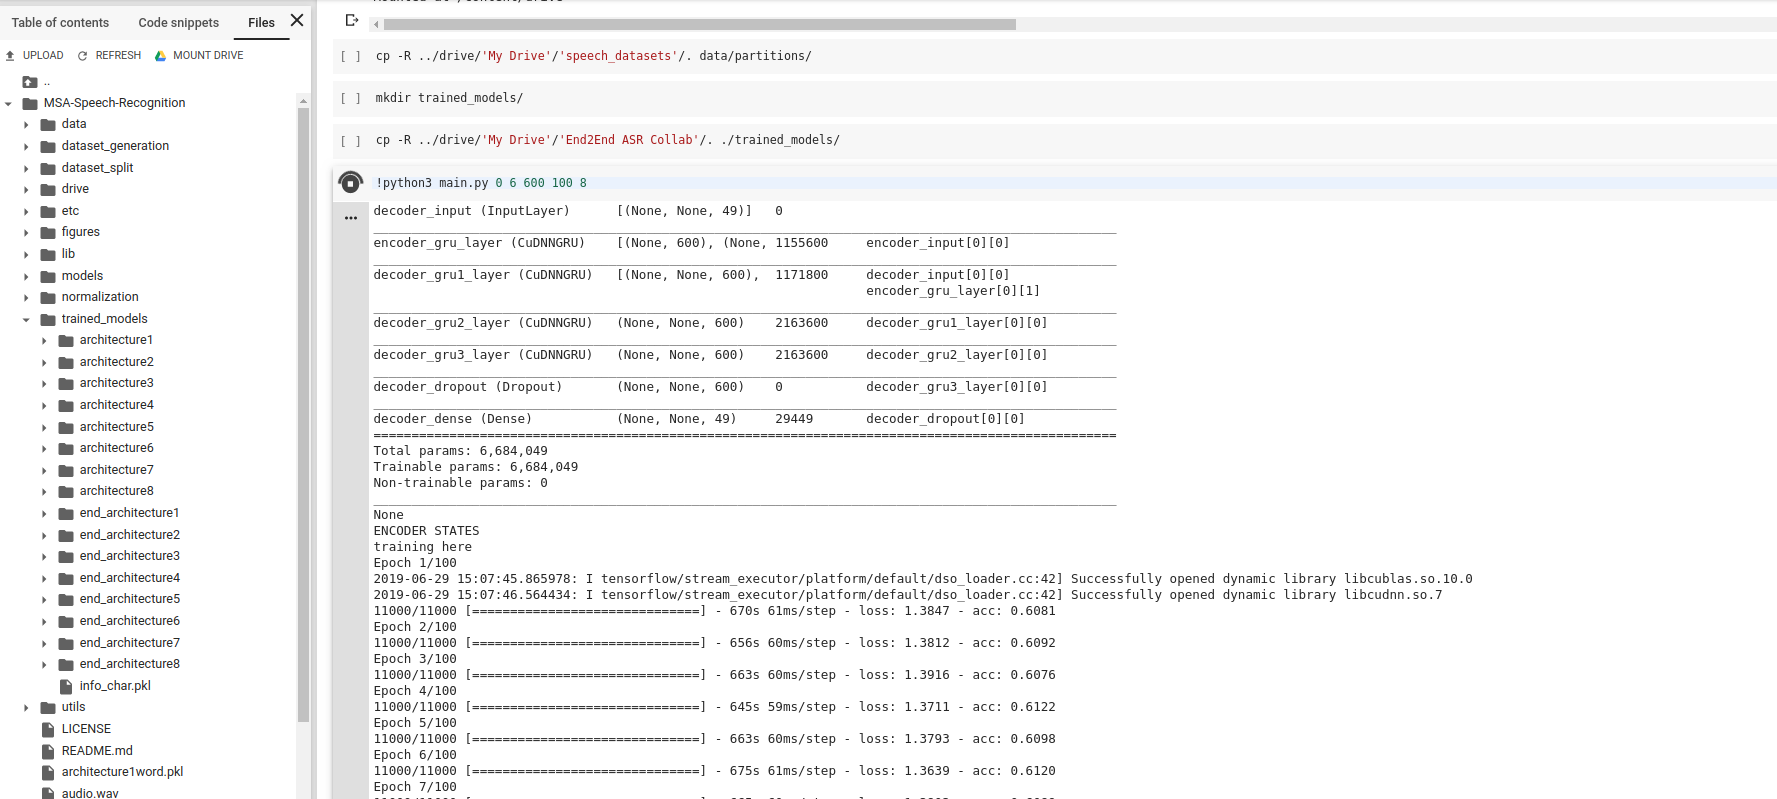
\includegraphics[width=450pt]{images/chap4/Collab.png}
    \caption{Exemple d'un environnement d'apprentissage avec Google Colaboratory}
    \label{Colab}
\end{figure}

Une difficulté que nous avons rencontrée est qu'une exécution à partir de Google Colaboratory ne dure que 12 heures et, une fois ce délai écoulé, toutes les données sur le disque sont effacées. Nous n'avions donc pas la possibilité d'enregistrer nos modèles pour poursuivre l'apprentissage. Afin de remédier à ce problème, nous sauvegardons le modèle ainsi que l'historique des courbes d'apprentissage sur Google Drive et ce, de manière automatique en implémentant la méthode \textit{on\_epoch\_end} dont l'appel s'effectue automatiquement à la fin de chaque itération.


\section{Apprentissage et discussion des résultats}
Nous passons à présent à l'apprentissage des modèles que nous avons définis dans la section \ref{apprentissage} de ce document. Pour la préparation des modèles et leurs apprentissages nous utilisons les couches que nous avons définies précédemment en variant les paramètres de celles-ci.

Pour l'apprentissage basé mots, chaque couche de sortie a sa propre exactitude et sa propre erreur. Pour une meilleure lecture des résultats nous calculons les moyennes des exactitudes et des erreurs sur les six premières couches de sortie car \textit{\%70} des mots du corpus ont une taille égale ou inférieure à six caractères, ce qui est assez représentatif. Nous avons choisi de calculer cette moyenne sur six caractères car seulement \textit{39\%} des mots ont cinq caractères ou moins. En plus de cela, au delà de six caractères les exactitudes sont très élevées car elles représentent les exactitudes des caractères de fin de mots. Prendre en compte les exactitudes de ces couches de sortie risquerait de biaiser la performance rapportée du système.

Nous présentons dans cette section les architectures pour chacun des modèles avec les meilleures performances au test sous forme de tableaux récapitulatifs et courbes de performances.

\subsection{Résultats d'apprentissage sur les différents corpus}
Nous présentons et discutons dans ce qui suit les résultats obtenus par les différentes architectures en nous basant sur les trois corpus suivants :
\begin{itemize}
    \item \textbf{Corpus d'essai} : ce corpus, que nous avons présenté dans la section \ref{corpus_essais}, est un corpus de six heures qui a pour but de tester le fonctionnement des différentes architectures. Nous effectuons l'apprentissage de cinq heures de dialogue et le test sur une heure.
    \item \textbf{60 heures de dialogue} : pour ce corpus nous effectuons l'apprentissage sur 52 heures de dialogue et le test sur huit heures. Ce corpus contient 35111 mots distincts, une taille de mots maximale de 15 caractères et un jeu de 42 caractères distincts.
    \item \textbf{260 heures de dialogue} : ce jeu de données contient 85532 mots distincts, une taille maximale de 16 caractères par mot pour un total de 49 caractères distincts. Nous divisons ces 260 heures de dialogue en 230 heures d'apprentissage et 30 heures de test.
\end{itemize}

\subsubsection{Apprentissage basé caractères}
Le tableau \ref{tableau1} résume les résultats de l'apprentissage en utilisant les couches unidirectionnelles avec les deux optimizers \textit{RMSprop} et \textit{Adagrad}. Le tableau \ref{tableau2} quant à lui résume les résultats obtenus avec les couches bidirectionnelles avec ces mêmes optimizers.

\begin{center}
\centering
    \begin{table}[H]
    \caption{Performances de l'apprentissage basé caractères avec couches unidirectionnelles}
    \label{tableau1}
    \resizebox{\textwidth}{!} & \makecell{71\%} & \makecell{75\%}\\
         \cline{6-9}
          &  &  &  &  & \makecell{Adagrad} & \makecell{31\%} & \makecell{69\%} & \makecell{88\%}\\
         \hline
         
          \multirow{2}*\makecell{six heures} & \multirow{2}*\makecell{2 Conv1D} & \multirow{2}*\makecell{1 GRU} &\multirow{2}*\makecell{2 GRU}  &\multirow{2}*\makecell{400} & \makecell{RMSprop} & \makecell{27\%} & \makecell{73\%}& \makecell{87\%}\\
         \cline{6-9}
          &  &  &  & & \makecell{Adagrad} & \makecell{32\%} & \makecell{68\%}& \makecell{87\%}\\
         \hline

         \multirow{2}*\makecell{60 heures} & \multirow{2}*\makecell{-} & \multirow{2}*\makecell{1 GRU} &\multirow{2}*\makecell{2 GRU}  & \multirow{2}*\makecell{500} & \makecell{RMSprop} & \makecell{42\%} &  \makecell{58\%}& \makecell{72\%}\\
         \cline{6-9}
          &  &  &  &  & \makecell{Adagrad} & \makecell{42\%} &   \makecell{58\%}& \makecell{72\%}\\
         \hline
          \multirow{2}*\makecell{60 heures} & \multirow{2}*\makecell{2 Conv1D} & \multirow{2}*\makecell{1 GRU} &\multirow{2}*\makecell{2 GRU}  & \multirow{2}*\makecell{400} & \makecell{RMSprop} & \makecell{40\%} & \makecell{70\%}& \makecell{73\%}\\
         \cline{6-9}
          &  &  & &  & \makecell{Adagrad} & \makecell{43\%} & \makecell{57\%}& \makecell{68\%}\\
         \hline
         
         \multirow{2}*\makecell{260 heures} & \multirow{2}*\makecell{-} & \multirow{2}*\makecell{1 GRU} &\multirow{2}*\makecell{3 GRU} &\multirow{2}*\makecell{550} & \makecell{RMSprop} & \makecell{51\%} & \makecell{49\%}& \makecell{54\%}\\
         \cline{6-9}
          &  &  & & & \makecell{Adagrad} & \makecell{68\%} & \makecell{32\%}& \makecell{41\%}\\
         \hline

         \multirow{2}*\makecell{260 heures} & \multirow{2}*\makecell{3 Conv1D} & \multirow{2}*\makecell{1 GRU} &\multirow{2}*\makecell{3 GRU} &\multirow{2}*\makecell{500} & \makecell{RMSprop} & \makecell{49\%} & \makecell{51\%}& \makecell{53\%}\\
         \cline{6-9}
          &  &  & & & \makecell{Adagrad} & \makecell{71\%} & \makecell{29\%}& \makecell{38\%}\\
         \hline
                
    \end{tabular}}
    \end{table}
\end{center}
\FloatBarrier

\begin{center}
\centering
    \begin{table}[H]
    \caption{Performances de l'apprentissage basé caractères avec couches bidirectionnelles}
    \label{tableau2}
    \resizebox{\textwidth}{!} & \makecell{74\%}& \makecell{89\%}\\
         \cline{6-9}
         
         \multirow{2}*\makecell{six heures} & \multirow{2}*\makecell{-} & \multirow{2}*\makecell{1 GRU} &\multirow{2}*\makecell{2 GRU}  &\multirow{2}*\makecell{500} & \makecell{Adagrad} &\makecell{26\%} & \makecell{74\%}& \makecell{91\%}\\
         \hline
         
          &  &  &  & & \makecell{RMSprop} & \makecell{22\%} & \makecell{78\%}& \makecell{89\%}\\
         \cline{6-9}
        
         \multirow{2}*\makecell{six heures} & \multirow{2}*\makecell{2 Conv1D} & \multirow{2}*\makecell{1 GRU} &\multirow{2}*\makecell{2 GRU}  &\multirow{2}*\makecell{400} & \makecell{Adagrad} & \makecell{25\%} & \makecell{75\%}& \makecell{89\%}\\
         \hline
         
          &  &  & & & \makecell{RMSprop} & \makecell{33\%} & \makecell{67\%}& \makecell{80\%}\\
         \cline{6-9}
         
         \multirow{2}*\makecell{60 heures} & \multirow{2}*\makecell{-} & \multirow{2}*\makecell{1 GRU} &\multirow{2}*\makecell{2 GRU} &\multirow{2}*\makecell{500} & \makecell{Adagrad} & \makecell{36\%} & \makecell{64\%}& \makecell{73\%}\\
         \hline
          &  &  & & & \makecell{RMSprop} & \makecell{34\%} & \makecell{77\%}& \makecell{79\%}\\
         \cline{6-9}
         
         \multirow{2}*\makecell{60 heures} & \multirow{2}*\makecell{2 Conv1D} & \multirow{2}*\makecell{1 GRU} &\multirow{2}*\makecell{2 GRU} &\multirow{2}*\makecell{400} & \makecell{Adagrad} & \makecell{37\%} & \makecell{73\%}& \makecell{70\%}\\
         \hline
           &  &  & &  & \makecell{RMSprop} & \makecell{49\%} & \makecell{51\%}& \makecell{54\%}\\
         \cline{6-9}
         
          \multirow{2}*\makecell{260 heures} & \multirow{2}*\makecell{-} & \multirow{2}*\makecell{1 GRU} &\multirow{2}*\makecell{3 GRU} & \multirow{2}*\makecell{550} & \makecell{Adagrad} & \makecell{64\%} & \makecell{36\%}& \makecell{43\%}\\
         \hline 
           &  &  &  &  & \makecell{RMSprop} & \makecell{49\%} & \makecell{51\%}& \makecell{56\%}\\
         \cline{6-9}

          \multirow{2}*\makecell{260 heures} & \multirow{2}*\makecell{3 Conv1D} & \multirow{2}*\makecell{1 GRU} &\multirow{2}*\makecell{3 GRU} & \multirow{2}*\makecell{500} & \makecell{Adagrad} & \makecell{68\%} & \makecell{32\%}& \makecell{41\%}\\
          \hline
    \end{tabular}}
    \end{table}
\end{center}
\FloatBarrier

\textbf{Discussion des résultats :} Nous remarquons tout de suite une grande différence entre les résultats obtenus pour chaque optimizer. La fonction \textit{Adagrad} présente des résultats nettement meilleurs que \textit{RMSprop}. Nous nous intéressons donc aux résultats obtenus avec l'utilisation de \textit{Adagrad}. Nous discutons ces résultats pour chaque corpus afin d'étudier l'évolution des performances des modèles avec l'augmentation du volume de données. Cette étude nous permettra de choisir, sur la base des résultats obtenus, le modèle adéquat pour l'apprentissage sur les 1200 heures de dialogue.

\begin{itemize}
    \item \textbf{Corpus d'essai (six heures de dialogue)} : nous ne pouvons donner une interprétation digne d'intérêt aux résultats obtenus à partir du corpus d'essai. En effet, pour une problématique aussi complexe que la reconnaissance de la parole en utilisant un modèle End-To-End, cinq heures de dialogue ne sont pas représentatives provoquent clairement un sous apprentissage. Ce corpus a été utilisé uniquement dans le but de tester le bon fonctionnement de nos modèles. Nous passons à l'apprentissage sur 60 heures de dialogue pour obtenir des résultats plus représentatifs. \\
    
    \item \textbf{60 heures de dialogue :} la première chose que nous notons est une hausse des résultats d'apprentissage par rapport au corpus d'essai. Lors de cet apprentissage, l'exactitude de l'apprentissage pour chacun des modèles à atteint les 99\%. Cependant comme le montre le tableau ci-dessus, les exactitudes de test ne dépassent pas les 43\% ce qui est un signe de sur-apprentissage. Nous expliquons cela par le faible nombre de données d'apprentissage pour une problématique aussi complexe que la reconnaissance de la parole. \\
    
    \item \textbf{260 heures de dialogue :} avec 260 heures de dialogue, nous notons une nette amélioration des résultats d'apprentissage en comparaison avec les 60 heures. L'augmentation du volume de données a permis de minimiser le sur-apprentissage. En effet, les exactitudes d'apprentissage sont de 75\% en moyenne. Nous remarquons également que le modèle à couches convolutionnelles a présenté les meilleurs résultats. Ceci est dû au traitement qu'effectuent les couches convolutionnelles sur les spectrogrammes avant que ceux-ci soient envoyés à l'encodeur. Notons cependant, que les modèles à couches bidirectionnelles ont présenté des résultats moin satisfaisants que les autres modèles. Ceci est dû à la quantité de données encore insuffisante ainsi qu'au temps que nous avons accordé aux apprentissages. Les modèles à couches bidirectionnelles prennent beaucoup plus de temps lors de l'apprentissage en comparaison aux autres modèles. Nous ne tentons pas d'aller plus loin dans l'apprentissage de ces modèles au vu de la limite de temps imparti pour la réalisation de ce projet. 
\end{itemize}

\subsubsection{Apprentissage basé mots}
Nous adoptons donc pour cet apprentissage l'architecture à plusieurs couches de sortie où chaque couche \textit{n} doit pouvoir reconnaître le \textit{nième} caractère d'un mot. Ce nombre de couches est égal au nombre maximum de caractères par mot. Au vu de la supériorité de la fonction \textit{Adagrad} par rapport à \textit{RMSprop}, pour notre problématique du moins, nous effectuons nos apprentissages avec \textit{Adagrad} uniquement. 

Comme pour l'apprentissage basé caractères, le tableau \ref{tableau3} concerne les couches unidirectionnelles quant au tableau \ref{tableau4}, il concerne les couches bidirectionnelles. Les résultats d'apprentissage sont les suivants.

\begin{center}
\centering
    \begin{table}[H]
    \caption{Performances de l'apprentissage basé mots avec couches unidirectionnelles}
    \label{tableau3}
    \resizebox{\textwidth}{!} & \makecell{78\%} & \makecell{82\%}\\
         \cline{2-8}
         
          & \makecell{2 Conv1D} & \makecell{1 GRU} &\makecell{2 GRU}  &\makecell{400} & \makecell{17\%} & \makecell{79\%}& \makecell{83\%}\\
         \hline
         
         \multirow{2}*\makecell{60 heures} & \makecell{-} & \makecell{1 GRU} &\makecell{2 GRU}  & \makecell{500} & \makecell{29\%} & \makecell{66\%}& \makecell{71\%}\\
         \cline{2-8}
         
           & \makecell{2 Conv1D} & \makecell{1 GRU} &\makecell{2 GRU}  & \makecell{400} & \makecell{31\%} & \makecell{67\%}& \makecell{69\%}\\
         \hline
         
         \multirow{2}*\makecell{260 heures} & \makecell{-} & \makecell{1 GRU} &\makecell{3 GRU} &\makecell{550} & \makecell{56\%} & \makecell{39\%}& \makecell{44\%}\\
         \cline{2-8}
          & \makecell{3 Conv1D} & \makecell{1 GRU} &\makecell{3 GRU} &\makecell{500} & \makecell{58\%} & \makecell{36\%}& \makecell{42\%}\\
         \hline
        
    \end{tabular}}
    \end{table}
\end{center}
\FloatBarrier
\begin{center}
\centering
    \begin{table}[H]
    \caption{Performances de l'apprentissage basé mots avec couches bidirectionnelles}
    \label{tableau4}
    \resizebox{\textwidth}{!} & \makecell{83\%}& \makecell{88\%}\\
         \cline{2-8}
         
         
          & \makecell{2 Conv1D} & \makecell{1 GRU} &\makecell{2 GRU}  &\makecell{400} & \makecell{14\%} & \makecell{83\%}& \makecell{86\%}\\
         \hline
         
         
         \multirow{2}*\makecell{60 heures} & \makecell{-} & \makecell{1 GRU} &\makecell{2 GRU} &\makecell{500} & \makecell{25\%} & \makecell{64\%}& \makecell{75\%}\\
         \cline{2-8}
          & \makecell{2 Conv1D} & \makecell{1 GRU} &\makecell{2 GRU} &\makecell{400} & \makecell{27\%} & \makecell{71\%}& \makecell{73\%}\\
         \hline
         
                 
          \multirow{2}*\makecell{260 heures} & \makecell{-} & \makecell{1 GRU} &\makecell{3 GRU} & \makecell{550} & \makecell{51\%} & \makecell{44\%}& \makecell{49\%}\\
         \cline{2-8} 
            & \makecell{3 Conv1D} & \makecell{1 GRU} &\makecell{3 GRU} & \makecell{500} & \makecell{55\%} & \makecell{39\%}& \makecell{45\%}\\
         \hline 
        
    \end{tabular}}
    \end{table}
\end{center}
\FloatBarrier

\textbf{Discussion des résultats} : Ici encore, nous discutons les résultats obtenus par les différents corpus à l'exception du corpus d'essai. 
\begin{itemize}

    \item \textbf{60 heures de dialogue} : nous remarquons une légère amélioration de la performance par rapport au corpus d'essai. Comme pour la reconnaissance basée caractères, l'exactitude d'apprentissage atteint les 99\% pour chaque modèle. Nous nous retrouvons donc dans une situation de sur-apprentissage. Nous justifions ce résultat par le nombre insuffisant de données d'apprentissage. En effet, pour l'apprentissage basé mots, le modèle a \textit{n} couches de sortie comme nous l'avons expliqué au début de cette section ce qui rend l'apprentissage sensiblement plus complexe. Nous ne pouvons espérer de bons résultats sans augmenter le volume de données. \\ 
    
    \item \textbf{260 heures de dialogue} : comme nous nous y attendions, nous notons une amélioration des performances qui est liée à l'augmentation du volume de données. Nous remarquons que le modèle à couches convolutionnelles a présenté les meilleurs résultats d'apprentissage même si l'exactitude n'est que de 58\% au test. Nous notons également un rapprochement entre l'exactitude d'apprentissage et de test minimisant ainsi le sur-apprentissage. Nous pensons que pour la reconnaissance basée mots, qui est de loin plus complexe que la reconnaissance basée caractères, un plus grand nombre de données est nécessaire. Nous étayons ce raisonnement par l'évolution de la performance lorsque nous sommes passé de 60 heures à 260 heures de dialogue. \\
\end{itemize}

Nous ne prenons pas la risque de lancer un apprentissage basé mots sur les 1200 heures de dialogue. Même si nous pensons que le modèle va enregistrer une performance nettement meilleure, nous ne pourrons en être sûrs sans expérimentation. 

L'apprentissage sur le corpus élargi, après un bref test, prend entre 15 et 20 minutes par itération d'où l'impossibilité de lancer un apprentissage sans être sûr de la performance que peut apporter le modèle. Nous ne savons pas si cette quantité de données suffirait au modèle. Il nous semble donc plus adéquat de lancer un apprentissage basé caractères en introduisant un modèle de langage pour améliorer encore plus la performance du modèle.

\subsection{Apprentissage sur le corpus élargi}
\subsubsection{Choix du modèle}
Notre choix quant au modèle que nous utilisons pour le développement de \textit{ASeR-System} s'est porté sur le modèle à couches convolutionnelles basé reconnaissance de caractères. Ce choix se justifie par les résultats prometteurs qu'a obtenu le modèle à couches convolutionnelles comparé aux autres modèles. Nous n'excluons pas la possibilité que les architectures à couches bidirectionnelles puissent présenter des résultats équivalents ou légèrement supérieurs aux résultats du modèle CNN mais nous ne pouvons déterminer à partir de quel volume de données ces modèles pourraient prendre le dessus sur le modèle CNN. Nous sommes également limité par la contrainte de temps car les modèles bidirectionnelles prennent plusieurs semaines d'apprentissage \cite{e2e4}.


\subsubsection{Apprentissage}
Après le pré-traitement des données, nous nous sommes retrouvés avec 860 heures de dialogue que nous avons divisées en 780 heures pour l'apprentissage et 80 heures pour le test. Ce corpus se compose de 153500 mots distincts et 49 caractères distincts. Le tableau \ref{perfappelargi} détaille l'architecture que nous avons mise en place. Il est à noter que les résultats ne sont pas finaux et que l'apprentissage est toujours en cours.

\begin{center}
\centering
    \begin{table}[H]
    \caption{Performance apprentissage modèle CNN sur le corpus élargi}
    \resizebox{\textwidth}{!} & \makecell{26\%} &\makecell{17\%}\\
         \hline
    \end{tabular}
    \label{perfappelargi}
    }
    \end{table}
\end{center}
\FloatBarrier

Les résultats obtenu avec le corpus élargi sont prometteurs. Nous estimons qu'en ajoutant du temps à l'apprentissage du modèle, celui-ci pourrait achever une meilleure performance. Augmenter le volume des données est également un garant de l'amélioration de la performance de ce modèle et est tout l'intérêt de l'utilisation de l'approche End-To-End.

\section{Environnement de développement pour la reconnaissance de la parole}
Nous présentons dans cette section l'implémentation de l'environnement de développement pour la reconnaissance de la parole ainsi que l'ensemble des paramétrages que nous avons mis en place. Pour le développement de cet environnement, nous nous sommes inspirés de la convention PEP8 en matière d'organisation pour simplifier à tout utilisateur l'intégration de nos modèles ou encore l'apprentissage de nouveaux modèles. Le schéma \ref{env_dev} résume l'organisation de l'environnement :

 \begin{figure}[H]
     \centering
     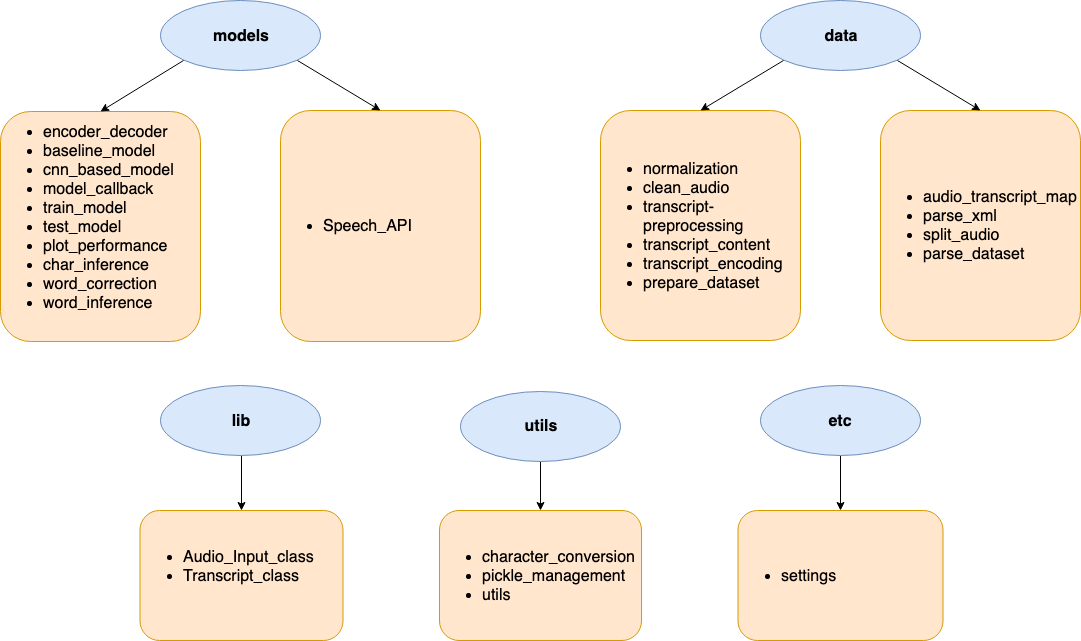
\includegraphics[height=275pt,width=400pt]{images/chap4/engine_packages.png}
     \caption{Disposition des packages de l'environnement de reconnaissance de la parole}
     \label{env_dev}
 \end{figure}

Nous avons implémenté l'environnement de développement de telle sorte à permettre à l'utilisateur d'utiliser chaque module indépendamment des autres modules. les modules sont les suivants : 
\begin{itemize}
    \item \textbf{models : } Ce module se divise en deux modules :
    \begin{enumerate}
        \item \textbf{Speech\_API} : module contenant un système de reconnaissance de la parole End-To-End prêt à intégrer à n'importe quelle application d'un simple appel de fonction.
        \item \textbf{Apprentissage :} Permettant d'effectuer l'apprentissage d'un modèle en second lieu. L'utilisateur a la liberté de modifier les couches utilisées pour l'apprentissage. Il est cependant à noter que tout changement dans les couches de l'architecture implique un changement au niveau de l'inférence. 
    \end{enumerate}
    \item \textbf{data :} Ce module se décompose à son tour en deux modules : 
        \begin{enumerate}
            \item \textbf{Génération de dataset :} Module semi-automatisé permettant de générer à partir d'enregistrements audio et transcriptions en format texte des fichiers Pickle, selon un nombre d'heures que peut définir l'utilisateur s'il le souhaite, associant à chaque enregistrement audio un spectrogramme MFCC ainsi que sa transcription. Ce module est semi-automatisé car les jeux de données ne sont pas toujours idéalement présentés (comme ce fut le cas pour le QCRI Speech Dataset).
            \item \textbf{Pré-traitement des données :} Ce module permet un certain nombre d'opérations sur les données tel que la normalisation des spectrogrammes, la suppression des enregistrements de mauvaise taille (d'une durée trop courte ou trop longue) ainsi que plusieurs types d'encodages des transcriptions comme nous l'avons présenté dans la section \ref{trans_preprocessing}. 
        \end{enumerate}
    \item \textbf{lib :} Module contenant les différentes classes utilisées.
    \item \textbf{utils :} Contenant différentes méthodes pour la gestion des répertoires et fichiers, conversion des caractères de Buckwalter vers l'arabe et vice versa, conversion binaire et bien d'autres.
    \item \textbf{etc :} Contenant les chemins relatifs et variables globales utilisées pour le pré-traitement et l'apprentissage.\\
\end{itemize}

Nous avons également mis en place une documentation détaillée concernant le fonctionnement de l'environnement de développement qui est disponible sur Github avec le système. Cette documentation est également disponible dans l'annexe de ce mémoire.

\section{Intégration du Système de questions-réponses}
Après avoir développé \textit{ASeR-System}, il est temps de le tester sur un vrai domaine d'application. Comme nous l'avons mentionné dans la section \ref{QASChap3}, nous avons choisi le domaine des systèmes de questions-réponses et plus particulièrement \textit{AFaQ-System}. \\

\textit{AFaQ-System} est basé sur un ensemble des paramètres que nous avons la possibilité de modifier pour effectuer différents tests. Ces paramètres sont les suivants : 
\begin{itemize}
    \item \textbf{--Mode :} définit le mode de recherche. Deux possibilités s'offrent à nous : le mode "Online" pour la recherche de réponses via le Web et le mode "Offline" dans le cadre de l'utilisation d'un corpus local.
    \item \textbf{--Source :} une chaîne de caractères précisant le chemin vers le corpus.
    \item \textbf{--Seuil :} représente le seuil de sélection des phrases pertinentes.
    \item \textbf{--SentenceSelection :} définit le nom du modèle à utiliser dans la phase de sélection des phrases.
    \item \textbf{--Model\_Path :} chaîne de caractères pour le chemin vers le modèle.
    \item \textbf{--NbrPassage :} le nombre des phrases à  sélectionner. \\
\end{itemize}
 
Dans notre cas, nous gardons les valeurs par défaut pour tous les paramètres cités sauf pour le \textbf{--mode} que nous mettons à Online pour ne pas être restreints à un corpus local. 

L'intégration \textit{AFaQ-System} avec \textit{ASeR-System} fut très simple, il nous a suffit d'appeler la fonction principale \textit{ArabicQuestionAnsweringSystem} du système de quesions-réponses en lui donnant en entrée la question qui représente la transcription de notre audio pour avoir la réponse en format texte.

\section{Application de ASeR-System sur un système de questions-réponses}
Afin de tester le bon fonctionnement de notre système de reconnaissance de la parole, nous avons développé une application Desktop avec la bibliothèque \textit{PyQT}. Cette application a pour objectif : 
\begin{itemize}
    \item d'effectuer un enregistrement sonore,
    \item d'utiliser la Speech\_API de \textit{ASeR-System} afin de générer la transcription de l'enregistrement sonore, 
    \item de trouver une réponse à la demande de l'enregistrement sonore en utilisant \textit{AFaQ-system}, et
    \item permettre à l'utilisateur de contribuer au projet en enregistrant un audio correspondant à une transcription afin d'augmenter la taille du corpus et ainsi, améliorer la performance de AeER-System.\\
\end{itemize}

Comme cette application est à but de test uniquement, nous avons développé une interface graphique simple et intuitive  permettant de réaliser les tâches ci-dessus. La figure \ref{main_window} présente la fenêtre principale de l'interface :

\begin{figure}[H]
     \centering
     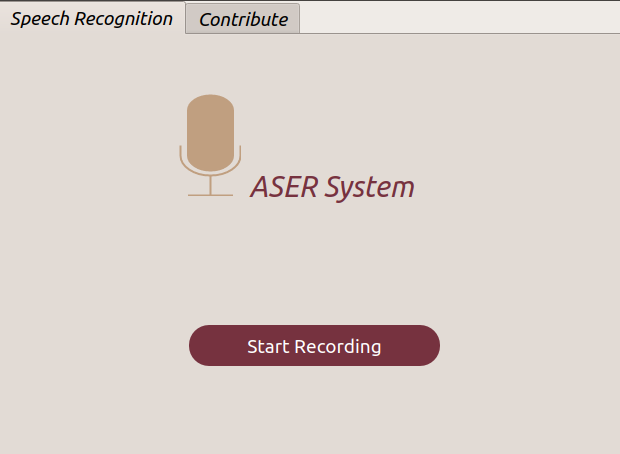
\includegraphics[height=250pt,width=430pt]{images/chap4/main_window.png}
     \caption{Fenêtre principale de l'application}
     \label{main_window}
 \end{figure}
 
 Ensuite, après avoir enregistré une question, \textit{ASeR-System} effectue la reconnaissance du dialogue contenu dans l'enregistrement et génère une transcription.  
 
\begin{figure}[H]
     \centering
     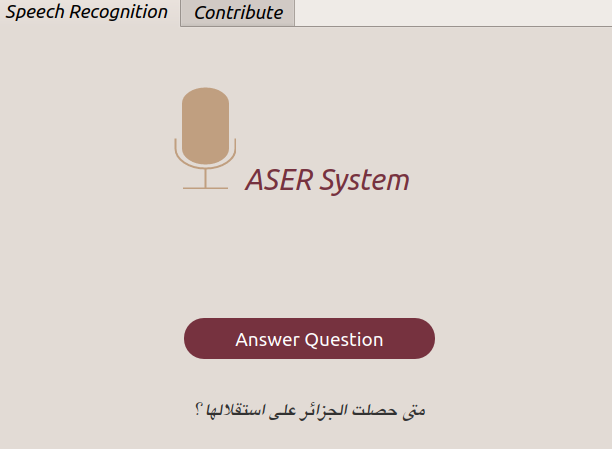
\includegraphics[height=250pt,width=430pt]{images/chap4/transcript_decoded.png}
     \caption{Affichage de la transcription}
     \label{}
 \end{figure}
 
Une fois la reconnaissance effectuée, l'utilisateur peut décider d'afficher une réponse à sa question et c'est là où nous faisons appel à \textit{AFaQ-System} pour trouver une réponse à cette question.
 
\begin{figure}[H]
     \centering
     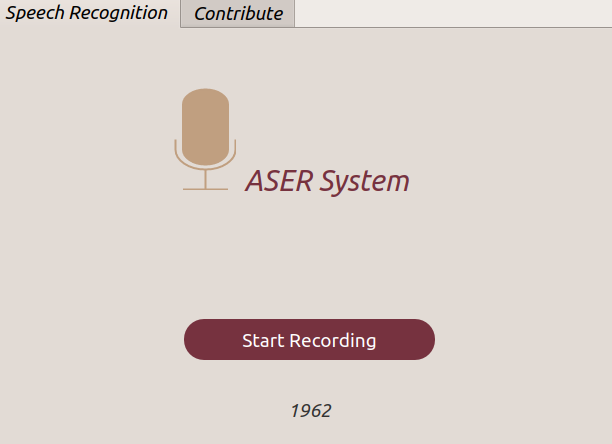
\includegraphics[height=250pt,width=430pt]{images/chap4/answer.png}
     \caption{Réponse à la question}
     \label{}
 \end{figure}
 
Nous avons également introduit un onglet contribution. Cette partie de l'application nous aidera à améliorer la performance de \textit{ASeR-System}. Nous générons aléatoirement des transcriptions à l'utilisateur pour que celui-ci enregistre un audio correspondant à ces transcriptions.

\begin{figure}[H]
     \centering
     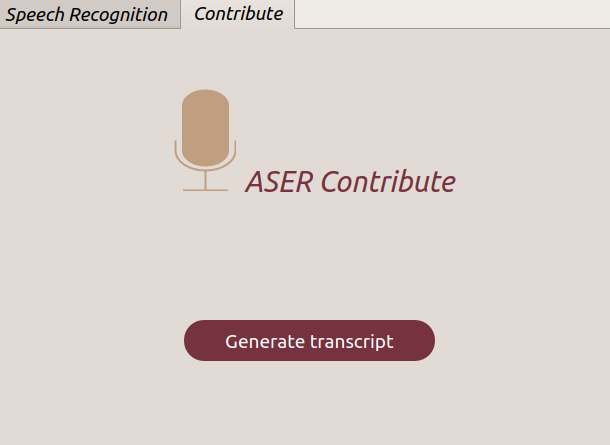
\includegraphics[height=250pt,width=430pt]{images/chap4/main_contribute.png}
     \caption{Onglet contribution de l'application}
     \label{}
 \end{figure}

Nous conservons ces enregistrements dans une base de données MySQL pour une utilisation future. 
 
 \begin{figure}[H]
     \centering
     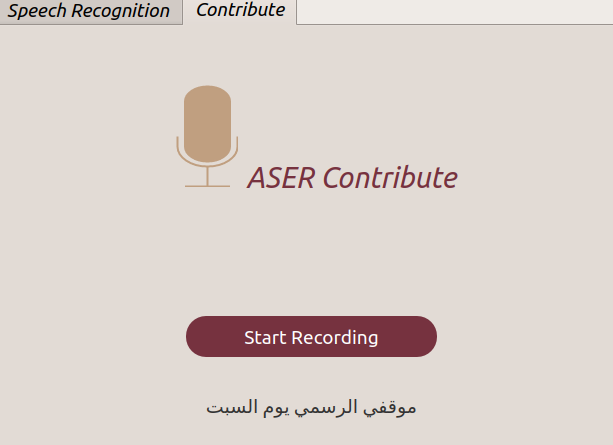
\includegraphics[height=250pt,width=430pt]{images/chap4/record_contribute.png}
     \caption{Génération d'une transcription pour la contribution}
     \label{}
 \end{figure}
 
Cette application est un exemple concret de l'utilisation du système de reconnaissance de la parole pour n'importe quel cas de figure tel qu'un système de questions-réponses.

\section{Conclusion}
À travers ce chapitre, nous avons présenté l'implémentation des différents modules de \textit{ASeR-System} en passant par l'environnement de travail, les différentes librairies utilisées mais aussi la génération des données d'apprentissage, la normalisation et la préparation des différents modèles. Nous avons également discuté les résultats d'apprentissage obtenus par les différents modèles et particulièrement le modèle final que nous avons choisi pour notre système de reconnaissance de la parole.

Nous avons conclu avec la présentation de l'application que nous avons réalisée pour tester \textit{ASeR-System} sur un système de questions-réponses. Cette application montre bien que notre environnement de développement permet de créer des systèmes de reconnaissance de la parole qui peuvent être utilisés dans tout type d'application de traitement automatique du langage naturel. 